\setcounter{secnumdepth}{-1}

\chapter{Introduction}

\section{Context}

We have been tasked to design a numeric controller for a given system which has to meet some requirements. The system is 
called \textit{DC motor and brake} and it consists of two current controlled motors connected to a brake trough a shaft. \\

Our objective is to send the best signal to the motors to ensure that:

\begin{enumerate}
    \item[$\bullet$] the shaft can reach any reasonnable speed in less than half a second
    \item[$\bullet$] the shaft's speed in maintained as smooth as possible
    \item[$\bullet$] the system can reject a step disturbance as fast as possible
    \item[$\bullet$] the shaft's speed can follow a feasible speed reference of $4 Hz$ from any feasible speed
\end{enumerate}

In addition to this, we could implement a strategy to reject various brake disturbances profile and magnitude, while 
maintaining the speed variations as smooth as possible.

\section{Plant description}

As explained in the introduction, the plant consists of two motors and one brake acting on the same shaft. There are 
three sensors available: one speed sensor and two position sensors.

\begin{figure}[H]
    \centering
    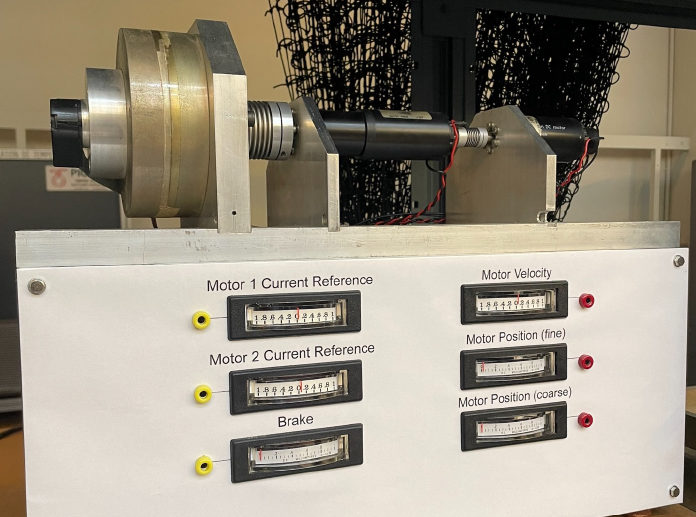
\includegraphics[height=\textheight/5]{Pictures/plant_picture.png}
    \caption{Picture of the plant}
\end{figure}

